\documentclass[../../main.tex]{subfiles}



\begin{document}

\section{Знакомство с деревьями}

\subsection{Описание деревьев}

Дерево это такой связный граф без циклов. Давайте посмотрим, как выглядят деревья:

Например, такое хорошее дерево:
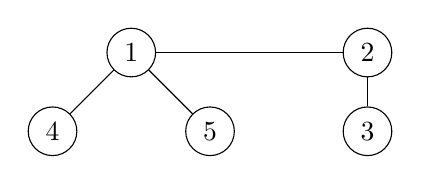
\begin{tikzpicture}[main/.style = {draw, circle},node distance={15mm}] 
    \node[main] (1) at (0,0){$1$}; 
    \node[main] (2) at (3,0){$2$}; 
    \node[main] (3) at (3, -1) {$3$};
    \node[main] (4) at (-1, -1) {$4$};
    \node[main] (5) at (1, -1) {$5$};
    \draw[-] (1) -> (2);
    \draw[-] (2) -> (3);
    \draw[-] (1) -> (4);
    \draw[-] (1) -> (5);
    %\draw (1) to [out=135,in=90,looseness=0.25] (6);
    %\draw[->] (2) -- node[midway, above right, sloped, pos=0.7] {$99$} (4);
    %\draw[->] (3) -> (4) node [midway, above] {$1$};
    %\draw[->] (1) -> (4) node [midway, left] {$100$};
    \end{tikzpicture} 

    Или такое:

    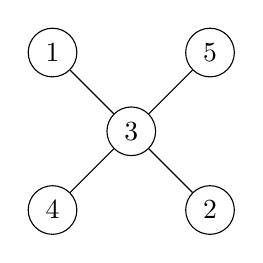
\begin{tikzpicture}[main/.style = {draw, circle},node distance={15mm}] 
        \node[main] (3) at (0,0){$3$}; 
        \node[main] (1) at (-1,1){$1$}; 
        \node[main] (5) at (1, 1) {$5$};
        \node[main] (4) at (-1, -1) {$4$};
        \node[main] (2) at (1, -1) {$2$};
        \draw[-] (3) -> (2);
        \draw[-] (3) -> (1);
        \draw[-] (3) -> (5);
        \draw[-] (3) -> (4);
        %\draw (1) to [out=135,in=90,looseness=0.25] (6);
        %\draw[->] (2) -- node[midway, above right, sloped, pos=0.7] {$99$} (4);
        %\draw[->] (3) -> (4) node [midway, above] {$1$};
        %\draw[->] (1) -> (4) node [midway, left] {$100$};
        \end{tikzpicture} 

    Еще один пример:

    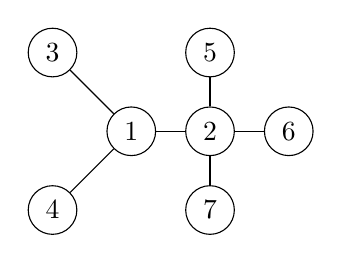
\begin{tikzpicture}[main/.style = {draw, circle},node distance={15mm}] 
        \node[main] (1) at (0,0){$1$}; 
        \node[main] (2) at (1,0){$2$}; 
        \node[main] (3) at (-1, 1) {$3$};
        \node[main] (4) at (-1, -1) {$4$};
        \node[main] (5) at (1, 1) {$5$};
        \node[main] (6) at (2, 0) {$6$};
        \node[main] (7) at (1, -1) {$7$};
        \draw[-] (1) -> (2);
        \draw[-] (1) -> (3);
        \draw[-] (1) -> (4);
        \draw[-] (2) -> (5);
        \draw[-] (2) -> (6);
        \draw[-] (2) -> (7);
        %\draw (1) to [out=135,in=90,looseness=0.25] (6);
        %\draw[->] (2) -- node[midway, above right, sloped, pos=0.7] {$99$} (4);
        %\draw[->] (3) -> (4) node [midway, above] {$1$};
        %\draw[->] (1) -> (4) node [midway, left] {$100$};
        \end{tikzpicture} 

Деревья интересны нам как минимум тем, что часто встречаются в различных олимпиадных и прикладных задачах. Итак, для начала нужно научиться понимать, 
что данный нам граф является деревом. Проговорим определение еще раз: 

\greenTitle{Определение}

\textbf{Деревом} называется связный граф без циклов.  

\greenTitle{Конец определения}

Таким образом, проверить граф на дерево будет очень просто, для этого нужно проверить граф на связность и проверить, что в нем нет цикла. Обе эти задачи решает алгоритм 
dfs'a, который вы все так знаете. Но на самом деле можно дать другое определение дереву: 

\greenTitle{Определение}

\textbf{Деревом} называется связный граф на $n$ вершинах с $n-1$ ребром. 

\greenTitle{Конец определения}

Таким образом, нам не нужно искать цикл в графе и можно воспользоваться более простой проверкой: проверить, что количество ребер равно $n-1$. Давайте докажем, что это так:

\begin{enumerate}
    \item В связном графе будет как минимум $n-1$ ребро. Почему это так: так как граф связный, рассмотрим любую вершину, пусть это вершина $1$. 
Теперь от нее можно будет дойти до любой другой вершины. Мы можем ориентировать ребра графа на пути из вершины $1$ во все другие, так в каждую вершину будет входить минимум одно ребро,
поэтому ребер в графе минимум $n-1$. 
    \item Предположим, что в граф можно добавить еще одно ребро $(x,y)$ таким образом, что цикла все еще не будет. Но тогда цикл точно образуется: 
    $1 \rightarrow x \rightarrow y \rightarrow 1$, ведь из-за связности графа существуют пути $1 \rightarrow x, y \rightarrow 1$. 
\end{enumerate}

Также можно пользоваться следующим определением: 

\greenTitle{Определение}

\textbf{Деревом} называется ацикличный граф на $n$ вершинах с $n-1$ ребром.

\greenTitle{Конец определения}

Однако как мы уже проговорили, легче проверить граф на связность. Для общего развития, давайте докажем и этот факт. 

\begin{enumerate}
    \item Предположим, что наш граф состоит из нескольких компонент связности, причем каждая из таких компонент -- дерево, так как 
    в каждой компоненте есть путь между любой парой вершин (иначе это не компонента связности) и там нет цикла, поэтому по определению это дерево. 
    \item Так как наш граф состоит из нескольких деревьев, то мы знаем количество ребер в каждом дереве, оно равно $a_i - 1$, 
    где $a_i$ это количество вершин в $i$-й компоненте. Но тогда количество ребер равно: $a_1 + a_2 + \ldots + a_k - k = n - 1$, то есть 
    $n - k = n - 1$, отсюда $k=1$. Да, $k$ это количество компонент связности графа, а так как в графе одна компонента связности, то он связный. 
\end{enumerate}

Итак, давайте напишем самым простым способом: проверим граф на связность и узнаем количество ребер: 

\subTitleStyle{Пример 1 (файл check)}

\ExampleFull{Sections/TreeBase/check.cpp}

\subTitleStyle{Конец примера 1}

\subsection{Пользуемся ацикличностью графа}

Так как все деревья ацикличны, то в них легко можно искать путь из какой-то вершины $x$ до всех остальных вершин. Для поиска 
длины пути мы используем \textit{bfs} или \textit{Деикстру}, но мы это делаем, так как в обычном графе могут быть циклы, в деревьях же цикла нет. 
\textbf{Если мы как-то дошли до вершины $x$, то это единственный способ дойти до нее}. Это дейсвительно так, ведь циклов нет. А какой алгоритм 
находит какой-то путь? Это делает алгоритм \textit{dfs}. Единственное: мы не хотим, чтобы алгоритм ходил по одному и тому же ребру несколько раз, поэтому 
мы запрещаем ходить в ту вершину, из которой вернулись.  

Итак, приведем сам код:

\subTitleStyle{Пример 2 (файл tree\_dist)}

\ExampleFull{Sections/TreeBase/tree_dist.cpp}

\subTitleStyle{Конец примера 2}

Давайте опишем, что делает функция \textit{dfs(x, dist, p)}: она принимает в себя текущую вершину $x$, расстояние от этой вершины до стартовой вершины $dist$, 
и также вершину $p$ откуда мы пришли в эту вершину, для стартовой вершины положим $p=-1$, поэтому, например, чтобы найти расстояние от вершины $1$ до всех других 
надо вызвать $dfs(1, 0, -1)$: стартовая вершина $1$, расстояние от нее до вершины $1$ равно $0$, а пришли мы из вершины $1$. 

\subsection{Подвешивание дерева}

Как вы заметили из прошлого кода, у каждой вершины подсчитывается также значение \textbf{родителя} --- такой вершины, из которой мы пришли в текущую в алгоритме \textit{dfs}'а.
Это действие называется подвешиванием дерева за корень, такое дерево уже называют \textbf{корневым} деревом. Так, у каждой вершины появляется глубина --- это расстояние до 
корня дерева. Может, звучит непонятно, но на рисунках все будет очевидно: возьмем следующее дерево: 

\begin{center}
    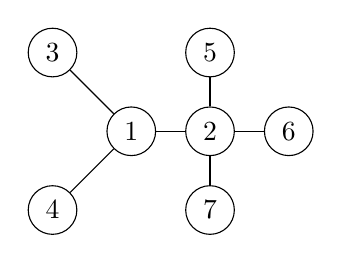
\begin{tikzpicture}[main/.style = {draw, circle},node distance={15mm}] 
        \node[main] (1) at (0,0){$1$}; 
        \node[main] (2) at (1,0){$2$}; 
        \node[main] (3) at (-1, 1) {$3$};
        \node[main] (4) at (-1, -1) {$4$};
        \node[main] (5) at (1, 1) {$5$};
        \node[main] (6) at (2, 0) {$6$};
        \node[main] (7) at (1, -1) {$7$};
        \draw[-] (1) -> (2);
        \draw[-] (1) -> (3);
        \draw[-] (1) -> (4);
        \draw[-] (2) -> (5);
        \draw[-] (2) -> (6);
        \draw[-] (2) -> (7);
        %\draw (1) to [out=135,in=90,looseness=0.25] (6);
        %\draw[->] (2) -- node[midway, above right, sloped, pos=0.7] {$99$} (4);
        %\draw[->] (3) -> (4) node [midway, above] {$1$};
        %\draw[->] (1) -> (4) node [midway, left] {$100$};
        \end{tikzpicture} 
\end{center}

Подвесим его за вершину $1$: 

\begin{center}

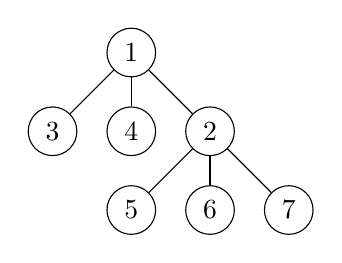
\begin{tikzpicture}[main/.style = {draw, circle},node distance={15mm}] 
    \node[main] (1) at (0,0){$1$}; 
    \node[main] (2) at (1,-1){$2$}; 
    \node[main] (3) at (-1, -1) {$3$};
    \node[main] (4) at (-0, -1) {$4$};
    \node[main] (5) at (0, -2) {$5$};
    \node[main] (6) at (1, -2) {$6$};
    \node[main] (7) at (2, -2) {$7$};
    \draw[-] (1) -> (2);
    \draw[-] (1) -> (3);
    \draw[-] (1) -> (4);
    \draw[-] (2) -> (5);
    \draw[-] (2) -> (6);
    \draw[-] (2) -> (7);
    %\draw (1) to [out=135,in=90,looseness=0.25] (6);
    %\draw[->] (2) -- node[midway, above right, sloped, pos=0.7] {$99$} (4);
    %\draw[->] (3) -> (4) node [midway, above] {$1$};
    %\draw[->] (1) -> (4) node [midway, left] {$100$};
    \end{tikzpicture} 

\end{center}

Давайте еще подвесим такое дерево за вершину $5$:

\begin{center}
    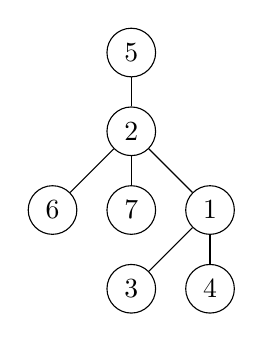
\begin{tikzpicture}[main/.style = {draw, circle},node distance={15mm}] 
        \node[main] (1) at (1,-2){$1$}; 
        \node[main] (2) at (0,-1){$2$}; 
        \node[main] (3) at (0, -3) {$3$};
        \node[main] (4) at (1, -3) {$4$};
        \node[main] (5) at (0, 0) {$5$};
        \node[main] (6) at (-1, -2) {$6$};
        \node[main] (7) at (0, -2) {$7$};
        \draw[-] (1) -> (2);
        \draw[-] (1) -> (3);
        \draw[-] (1) -> (4);
        \draw[-] (2) -> (5);
        \draw[-] (2) -> (6);
        \draw[-] (2) -> (7);
        %\draw (1) to [out=135,in=90,looseness=0.25] (6);
        %\draw[->] (2) -- node[midway, above right, sloped, pos=0.7] {$99$} (4);
        %\draw[->] (3) -> (4) node [midway, above] {$1$};
        %\draw[->] (1) -> (4) node [midway, left] {$100$};
        \end{tikzpicture} 
\end{center}

\begin{enumerate}
    \item Хоть это одно и то же дерево, но воспринимается как будто немного по-другому. 
    \item Обратите внимание, что вершины дерева ложатся по <<слоям>>, а именно по глубинам вершин. 
    \item Такие деревья называют \textbf{корневыми} или \textbf{подвешенными}. Выделенную вершину называют \textbf{корнем}. Напимер, первое дерево это корневое дерево с корнем $1$, а второе --- с корнем $t$.
    \item Для корневых и некоторневых деревьев отличают некоторые определения, об этом подробнее будем говорить потом.
\end{enumerate}

Подвешивание дерева бывает полезно в некоторых задачах, когда мы задаем дереву некую структуру. 

\subsection{Некоторые обозначения корневых деревьев}

Здесь приведем пару определений и обозначений, для примера будем использовать уже знакомое корневое дерево:

\begin{center}
    \begin{center}
        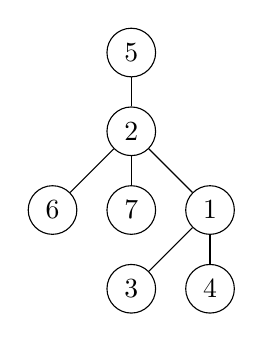
\begin{tikzpicture}[main/.style = {draw, circle},node distance={15mm}] 
            \node[main] (1) at (1,-2){$1$}; 
            \node[main] (2) at (0,-1){$2$}; 
            \node[main] (3) at (0, -3) {$3$};
            \node[main] (4) at (1, -3) {$4$};
            \node[main] (5) at (0, 0) {$5$};
            \node[main] (6) at (-1, -2) {$6$};
            \node[main] (7) at (0, -2) {$7$};
            \draw[-] (1) -> (2);
            \draw[-] (1) -> (3);
            \draw[-] (1) -> (4);
            \draw[-] (2) -> (5);
            \draw[-] (2) -> (6);
            \draw[-] (2) -> (7);
            %\draw (1) to [out=135,in=90,looseness=0.25] (6);
            %\draw[->] (2) -- node[midway, above right, sloped, pos=0.7] {$99$} (4);
            %\draw[->] (3) -> (4) node [midway, above] {$1$};
            %\draw[->] (1) -> (4) node [midway, left] {$100$};
            \end{tikzpicture} 
    \end{center}
\end{center}

\begin{enumerate}
    \item Обозначим вершину-корень дерева. Теперь \textbf{мысленно} ориентируем ребра от корня дерева вниз до всех вершин дерева. 
    \item Если в вершину $y$ приходит ребро из вершины $x$, то говорят что $x$ \textbf{родитель} $y$. Например, для вершины $1$ родителем является вершина $2$. 
    А для вершины $2$ родителем является вершина $5$.
    \item Обычно родителя корня не определяют или определяют числом $-1$. 
    \item Если вершина $x$ является \textbf{родителем} вершины $y$, то говорят что $y$ \textbf{ребенок} $x$. Например, у вершины $2$ есть дети $6,7,1$. 
    А у вершин $6,7,3,4$ детей нет. 
    \item Листом \textbf{дерева} называется вершина со степенью $1$. Иными словами, всего одно ребро инцидентно данной вершине. На рисунке 
    это вершины $3,4,5,6,7$.
    \item Однако листом \textbf{корневого} дерева называется такая вершина, у которой нет детей. На рисунке 
    это вершины $3,4,6,7$. Обратите внимание, вершина $5$ листом не является. 
    \item Иногда корневое дерево задают не с помощью списка ребер, для данного дерева он, кстати, может являться таким: $[(2,5), (2,6), (2,7), (1,2), (1,3), (1,4)]$. 
    Но задают с помощью списка родителей для каждой вершины, обозначая для корня значение $-1$. Например, данное дерево 
    можно задать так: $[2, 5, 1, 1, -1, 2, 2]$. Например, родитель вершины $1$ это $2$, родитель вершины $2$ это $5$, родитель вершины $3$ это $1$, родитель вершины $4$ это $1$,
    родитель вершины $5$ это $-1$, значит, $5$ --- корень дерева. 
    Так можно задать дерево не $2(n-1)$ числами, а всего $n$ числами.
    \item Говорят, что вершина $x$ предок вершины $y$, если поднимаясь по родителям из $y$ можно добраться до $x$. Иными словами, это все вершины до корня дерева из текущей вершины. 
    Например, для вершины $3$ предками являются $1,2,5$. 
    \item Общий предок двух вершин это такая вершина, что является предком и первой, и второй вершиной. Например, у вершин $(6,3)$ есть общие предки $(2,5)$. 
    \item Наименьший общий предок двух вершин, это такая вершина, что ее родитель не является общим предком. Например, у вершин $(6,3)$ наименьший общий предок это $2$. 
\end{enumerate}

Приведем алгоритм dfs, который рассчитывает родителя для каждой вершины и сохраняет в массив \textit{parent}:

\subTitleStyle{Пример 3 (файл parent.cpp)}

\ExampleFull{Sections/TreeBase/parent.cpp}

\subTitleStyle{Конец примера 3}

Как и в обычном графе, в дереве можно найти путь между двумя вершинами, используя \textit{dfs}, однако здесь нам опять же не нужен массив \textit{color} для 
отметки непосещенных вершин:

\subTitleStyle{Пример 4 (файл path.cpp)}

\ExampleFull{Sections/TreeBase/parent.cpp}

\subTitleStyle{Конец примера 4}

\subsection{Подведение итогов}

\begin{enumerate}[label=\Roman*]
    \item В решении задач на деревьях пользуйтесь тем фактом, что в дереве нет циклов.
    \item Старайтесь всегда рассматривать корневые деревья, создавая некую иерархию в графе. Это более подробно будет в следующих занятиях. 
    \item Используйте алгоритм dfs для работы с деревьями, здесь не нужна ни Деикстра, ни бфс.
\end{enumerate}

\end{document}
